
\documentclass[11pt]{article}
%%%%%%%%%%%%%%%%%%%%%%%%%%%%%%%%
\usepackage{amsmath}
\usepackage{amsthm}
\usepackage{footnote}
\usepackage{fancyhdr}
\usepackage{amssymb}
\usepackage{tikz}
\usepackage{listings}
\usepackage{color}
\usepackage{graphicx}
\usepackage{subcaption}


\definecolor{codegreen}{rgb}{0,0.6,0}
\definecolor{codegray}{rgb}{0.5,0.5,0.5}
\definecolor{codepurple}{rgb}{0.58,0,0.82}
\definecolor{backcolour}{rgb}{0.95,0.95,0.92}

\lstdefinestyle{mystyle}{
	backgroundcolor=\color{backcolour},   
	commentstyle=\color{codegreen},
	keywordstyle=\color{magenta},
	numberstyle=\tiny\color{codegray},
	stringstyle=\color{codepurple},
	basicstyle=\footnotesize,
	breakatwhitespace=false,         
	breaklines=true,                 
	captionpos=b,                    
	keepspaces=true,                 
	numbers=left,                    
	numbersep=5pt,                  
	showspaces=false,                
	showstringspaces=false,
	showtabs=false,                  
	tabsize=2
}

\lstset{style=mystyle}

\usepackage{hyperref}
\hypersetup{
	colorlinks=true,
	linkcolor=blue,
	filecolor=magenta,      
	urlcolor=cyan,
}

\theoremstyle{plain}
\newtheorem*{theorem*}{Theorem}
\newtheorem*{notation*}{Notation}
\newtheorem*{algorithm*}{Algorithm}
\newtheorem*{remark*}{Remark}
\newtheorem{theorem}{Theorem}[section]
\newtheorem{algorithm}{Algorithm}[section]
\newtheorem{axiom}[theorem]{Axiom}
\newtheorem{claim}[theorem]{Claim}
\newtheorem{corollary}[theorem]{Corollary}
\newtheorem{definition}[theorem]{Definition}
\newtheorem{example}[theorem]{Example}
\newtheorem{lemma}[theorem]{Lemma}
\newtheorem{notation}[theorem]{Notation}
\newtheorem{problem}[theorem]{Problem}
\newtheorem{proposition}[theorem]{Proposition}
\newtheorem{remark}[theorem]{Remark}
\newtheorem{summary}[theorem]{Summary}
\newtheorem{assumption}{Assumption}[section]

\DeclareMathOperator*{\argmax}{arg\,max}
\DeclareMathOperator*{\E}{\mathbb{E}}
\let\Pr\relax
\DeclareMathOperator*{\Pr}{\mathbb{P}}


\begin{document}

\title{Report for Independent Study\\
Deep Learning and Part-of-speech Tagging}
\author{Min Chen}
\date{\today}
\maketitle
\thispagestyle{fancy}
\lhead{Deep Learning and POS}
\rhead{IUB Summer 2018}
\rfoot{Page \thepage}

\begin{abstract}
	
This is the report for an independent study with Prof. Damir Cavar at Indiana 
University Bloomington for the Summer Semester 2018. The independent 
study is conducted in several parts throughout the summer including reading 
groups led by Prof. Damir, guided reading over reference books, slides and 
papers, as well as hands-on coding for part-of-speech tagging using deep 
learning techniques. 

\end{abstract}
\pagebreak
\tableofcontents
\listoffigures
\listoftables
\pagebreak


\section{Introduction}

Deep learning has been a hot topic in computer science especially artificial 
intelligence (AI) in recent years, especially after the five-game Go match 
between 18-time world champion Lee Sedol and AlphaGo, a computer Go 
program developed by Google DeepMind. Deep learning or more specifically, 
deep neural networks has been applied to most if not all AI applications such 
as computer vision and natural language processing. 

Prof. Damir Cavar at Indiana University taught a course named Deep Learning 
and NLP in Spring 2017 and I did not have chance to participate. Since the 
techniques and applications of deep learning is so interesting and important, 
I decided to participate in an independent study with Prof. Cavar, focusing on 
deep learning with applications on natural language processing. 

The whole process of independent study consists of several components: 
\begin{enumerate}
	\item Reading group regarding linear algebra and quantum algorithm
	\item Project group regarding open information extraction (openIE) 
	\item Individual study and meeting with Prof. Cavar regarding deep learning 
	basics and NLP applications
\end{enumerate}
In this report, I will briefly summarize the knowledge and results from the last 
component listed, i.e. deep learning basics and NLP applications, in particular 
my experiments of part-of-speech tagging using deep learning techniques I 
learnt. 


\paragraph{Outline}The report is structured in the following way: 
Section \ref{s:pre} lists some basic knowledge and tools which are 
considered as preliminary to deep neural network models. The author spent 
two weeks reviewing materials regarding these preliminaries before actually 
started working on deep learning materials. Techniques and knowledge of 
deep neural networks that the author learnt are summarized in Section 
\ref{s:dnns}.  Section \ref{s:w2v} talks about 
word embeddings (word2vec), a warm up application of neural networks in 
natural language processing. This is also used in later sections as an input to 
train POS taggers. Section \ref{s:pos-sklearn} focuses on using the machine 
learning library scikit-learn (in Python)for POS tagging on Brown Corpus and 
Part of the Penn Tree Bank. The author tried two methods. One uses 
basic token level features and the other uses word2vec. Section \ref{s:LSTM} 
discusses the use of Keras deep learning library and 
apply the model of Bidirectional Long Short-Term Memory Recurrent Neural 
Network for POS tagging, which is more accurate and efficient than the 
previous attempts. Finally, Section \ref{s:conclusion} concludes and lists 
several questions for future research and discussion. 


\paragraph{Materials and Resources }
There are several important sources that the author read and referenced 
when studying this topic and writing the report. 
\begin{itemize}
	\item The deep learning text book by Goodfellow, Bengio and Courville 
	\cite{Goodfellow-et-al-2016}. I also refers to the website links and youtube 
	videos provided by Goodfellow regarding the materials of the book to get 
	a better understanding. 
	\item Course materials by Prof. Damir Cavar \cite{Cavar2018-i665} 
	including slides from the Stanford NLP course \cite{CS224}. 
	\item Guidance on POS tagging with BLSTM-RNN including a paper 
	\cite{Wang2015PartofSpeechTW}, a github repository with code examples 
	and explanation \cite{aneesh-joshi-LSTM-POS-Tagger} and a blog 
	explaining Long Short-Term Memory RNN \cite{olah-blog-lstm}.
	\item Other notes, materials and papers used, will be acknowledged and 
	cited in later sections.
\end{itemize}

\section{Deep Learning Preliminaries Summary}
\label{s:pre}

This section lists several of the preliminary piece of knowledge of deep 
learning models and techniques, which are reviewed in details by the author 
before step into the world of deep neural networks. The readings referenced 
including the first five chapters of the deep learning text book 
\cite{Goodfellow-et-al-2016} and some of the pdf materials by Zico Kolter. 

\subsection{Probability Theory}

Many machine learning algorithm including deep neural networks all have 
probability theory as the theoretic foundation. Some common distributions 
are widely used such as Bernoulli, Multinoulli, Guassian. For example, in a 
task of multi-class classification, we are trying to learn a Multinoulli 
distribution from the data. 

Estimation theory is also applied when we try to maximize (or minimize) the 
objective functions, the core concepts involve maximum likelihood 
estimation, maximum a posteriori estimation, mean squared errors etc. 

Finally, information theory especially Shannon entropy plays an important 
role defining the loss (objective) functions of machine learning models. In 
fact, cross-entropy, which is closely related to Kullback-Leibler divergence, is 
often used as the loss function for multi-classes classification. This could be 
treated as an interpretation for the maximum likelihood estimator. Suppose 
we are maximizing the log-likelihood function regarding some parameter 
$\theta$, using data $x_i$'s
\[
\hat{\theta}_{ML}=\argmax_{\theta} \sum_{i=1}^{m} \log P_{model}(x_i; \theta)
\]
The summation could be viewed as an expectation with respect to the 
empirical distribution $P_{data}$. Hence we got the following equivalent 
expression: 
\[
\hat{\theta}_{ML}=\argmax_{\theta} \E_{x\sim P_{data}} \log P_{model}(x; 
\theta)
\]
If we use KL divergence to describe the dissimilarity between the empirical 
distribution $P_{data}$ and the real underlying data generating process 
$P_{model}$, we have:
\[
D_{KL}(P_{data}||P_{model})=\E_{x\sim P_{data}} (\log P_{data}(x) - \log 
P_{model}(x))
\]
Since $\E_{x\sim P_{data}} \log P_{data}(x)$ is constant, getting the maximum 
likelihood estimator is equivalent to minimize:
\[
-\E_{x\sim P_{data}} \log P_{model}(x)
\]
which is the cross-entropy between empirical 
distribution and the real underlying data generating process.

Goodfellow also noted that Any loss consisting of a negative log-likelihood is 
a cross-entropy between the empirical distribution defined by the training set 
and the probability distribution defined by the model. For example, mean 
squared error is the cross-entropy between the empirical distribution and a 
Gaussian model \cite{Goodfellow-et-al-2016}. 

\subsection{Linear Algebra}

Linear Algebra is very important for machine learning especially deep neural 
networks. In fact, many neural network models are in essence just complex 
matrix multiplications. The word2vec model for word embeddings (explained 
in Section \ref{s:w2v}) is a good example. 

To better understand the materials on deep learning, key concepts of linear 
algebra including matrix multiplication, linear dependence, norm, 
eigen-decomposition, trace and determinant need to be reviewed and 
well-understood. 

While the topics listed above are typically covered in a standard course on 
linear algebra, one topic that does not seem to be covered very often (but 
used extensively in deep learning) is the extension of calculus to the vector 
setting. I referred to the paper by Terence Parr and Jeremy Howard to get a 
good summary of the core concept and notations of matrix calculus 
\cite{DBLP:journals/corr/abs-1802-01528}. This piece of knowledge is very 
important for derivation of most of the theoretical models in neural networks 
as well as understanding the core concept of training them: gradient 
descent and back propagation. 

Several formula that are useful for remembering:
\begin{itemize}
	\item $\nabla_x b^{T}x = b$ ($x$ and $b$ are vectors)
	\item $\nabla_x x^{A}x = 2Ax$ ($A$ is a symmetric matrix)
	\item $\nabla_x^2 x^{A}x = 2A$ ($A$ is a symmetric matrix)
	\item Let $f$ be some loss function and $\frac{\partial f}{\partial C}=G$ 
	where $C=AB$ then the chain rule implies $\frac{\partial f}{\partial 
	A}=\frac{\partial f}{\partial C}B^{T}=GB^{T}$. 
\end{itemize}

\subsection{Convex Optimization}
Convex optimization is a very important area in optimization, economics and 
many other disciplines. In this part, I reviewed several general 
techniques/concepts: in unconstrained optimization problems, first-order 
gradient descent, second-order optimization (Newton's method using 
Hessian matrix). In constrained problems with equality and/or in-equality 
constraints, Lagrangian or Karush-Kun-Tucker method is used. 

The importance of convexity is the guarantee of global minimum and fast 
convergence using gradient-based algorithms regardless of initial state. 
However, in general settings, we do not have global convexity or concavity. 
There may be many local maximum, local minimum, saddle points etc. 

\subsection{Machine Learning basics}

In this part, the author reviewed several basic machine learning algorithms 
and general techniques in designing and training the models followed by 
Chapter 5 of the Deep Learning text book \cite{Goodfellow-et-al-2016}. 

Basic algorithms include supervised learning algorithms such as support 
vector machines, decision trees, logistic regression, and unsupervised 
learning algorithms such as principle component analysis, and k-means 
clustering. 

Useful techniques in design and training include concepts of capacity, 
over-fitting and under-fitting and use of hyper-parameters and validation 
sets. A key method in training is stochastic gradient descent, which is more 
efficient and less memory-consuming than the "deterministic" version. 

\section{Deep Neural Network Summary}
\label{s:dnns}

This section summarizes basic knowledge and practices in modern deep 
networks following the chapters 6 to 10 in Deep Learning book. 

\subsection{Deep Feedforward Networks}
Deep feedforward network can be also referred to as feedforward neural 
networks or multilayer perceptrons (MLPs). There is no other obvious 
difference between deep forward network and the common neural network 
other than the fact that deep network may have more hidden layers (i.e. 
deeper). 

Feedforward networks are typically represented by composing together many 
different functions, where the parameters to be learnt are often called 
weights. Back-propagation algorithm is used to train the model and learn the 
weights. The algorithm is basically a big chain rule calculating the partial 
derivatives of the loss function with respect to all the weights in previous 
layers. 

The book \cite{Goodfellow-et-al-2016} uses an entire chapter discussing 
regularization for deep learning and another chapter for optimization in 
training feedforward networks. These techniques are very practical and 
widely used in different deep learning libraries such as scikit-learn and keras. 

\subsection{Convolutional Neural Network}
Convolutional neural networks (CNN) are a specialized kind of neural network 
for processing data that has a known grid-like topology. Examples include 
time-series data (1-D grid), image data (2-D grid of pixels) and volumetric 
data (3-D grid). There are three main types of layers that are often used to 
build CNN architectures: convolutional Layer, pooling Layer, and 
fully-connected Layer. However, since the author's focus is on natural 
language processing, which is not grid-like but sequence-like data, the more 
relevant model is recurrent neural networks (RNN).

\subsection{Recurrent Neural Network}
A recurrent neural network (RNN) is specialized for processing a sequence of 
values. The extension for feedforward network to recurrent network involves 
the idea of parameter sharing, which makes it possible to apply the model to 
sequences of different length and generalize across them. 

One simple illustration of RNN is in Figure \ref{fg:unroll-rnn}, where $A$ is 
some structure of network layers, for example a simple hidden layer or 
composition of several hidden layers. The model takes a sequence of inputs 
$x_i$, feed to the same network structure at each step and produce $h_i$ as 
outputs. The left-hand side is a compact way of the RNN before unrolling. 

\begin{figure}[!ht]
	\centering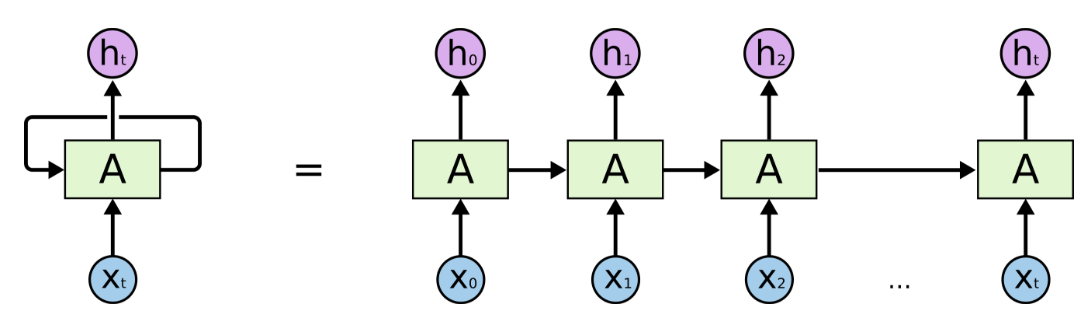
\includegraphics[width=\columnwidth]{images/unfold-rnn.png}
	\caption{An Unrolled Recurrent Neural Network 
	}\label{fg:unroll-rnn}\cite{olah-blog-lstm}
\end{figure}

In previous example, the network is one-directional, i.e. the state at time $t$ 
captures only information from the past, $t-1$, $t-2$,... However, sometimes 
use a bidirectional RNN to allow the current state depends on both previous 
and post information. In particular: ``using bidirectional will run inputs in two 
ways, one from past to future and one from future to past and what differs 
this approach from unidirectional is that in the RNN that runs backwards you 
preserve information from the future and using the two hidden states 
combined you are able in any point in time to preserve information from both 
past and future. Because of their ability to approach a unit from both the 
directions, they tend to understand context better'' 
\cite{aneesh-joshi-LSTM-POS-Tagger}. This could be illustrated in Figure 
\ref{fg:bi-rnn}, where $h^{(t)}$ are states moving forward through time and 
$g^{(t)}$ are states moving backward. The output at each time point is 
depending on both states. 
\begin{figure}[!ht]
	\centering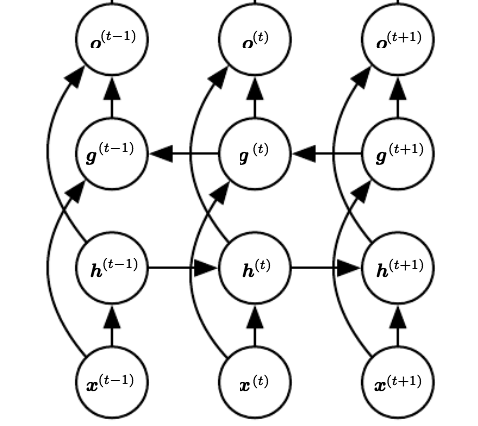
\includegraphics[width=0.7\columnwidth]{images/bi-rnn.png}
	\caption{Bidirectional Recurrent Neural Network 
	}\label{fg:bi-rnn}	\cite{Goodfellow-et-al-2016}
\end{figure}

For the Part-of-speech tagging in Section \ref{s:LSTM}, a special RNN is 
used: Long Short-Term Memory Recurrent Neural Network. The details will be 
discussed in that section. 


\section{Warm-up: Word Embeddings and Word2vec}
\label{s:w2v}
This section talks about word embeddings, ``which is the collective name for 
a set of language modeling and feature learning techniques in natural 
language processing (NLP) where words or phrases from the vocabulary are 
mapped to vectors of real numbers. Conceptually it involves a mathematical 
embedding from a space with one dimension per word to a continuous vector 
space with a much lower dimension'' \cite{wiki-wordembedding}. The 
word2vec is a model used to produce word embeddings. It is interesting in 
two ways. First, word2vec itself is a two-layer neural networks that are 
trained to reconstruct linguistic contexts of words, which can be think of as 
a simple application of feedforward networks. Second, using the resulting 
vectors as features for further NLP tasks is considered better in many cases 
due to less human supervised feature engineering. 

\subsection{Model}
The model of word2vec is a two-layer neural networks with one hidden layer 
and one output layer. Given a specific word in the middle of a sentence (the 
input word), the network is going to predict the probability for every word in 
the vocabulary of being the context word i.e. within a certain window of the 
input word. A typical window size is 5, which means 5 words behind and 5 
words ahead of the input word are considered as the context.

The network is trained by feeding word pairs found in training documents 
that are within the window size. Let us assume that the vocabulary is 10000. 
The structure of the network is illustrated in 
Figure \ref{fg:w2v-structure}. 

\begin{figure}[!ht]
	\centering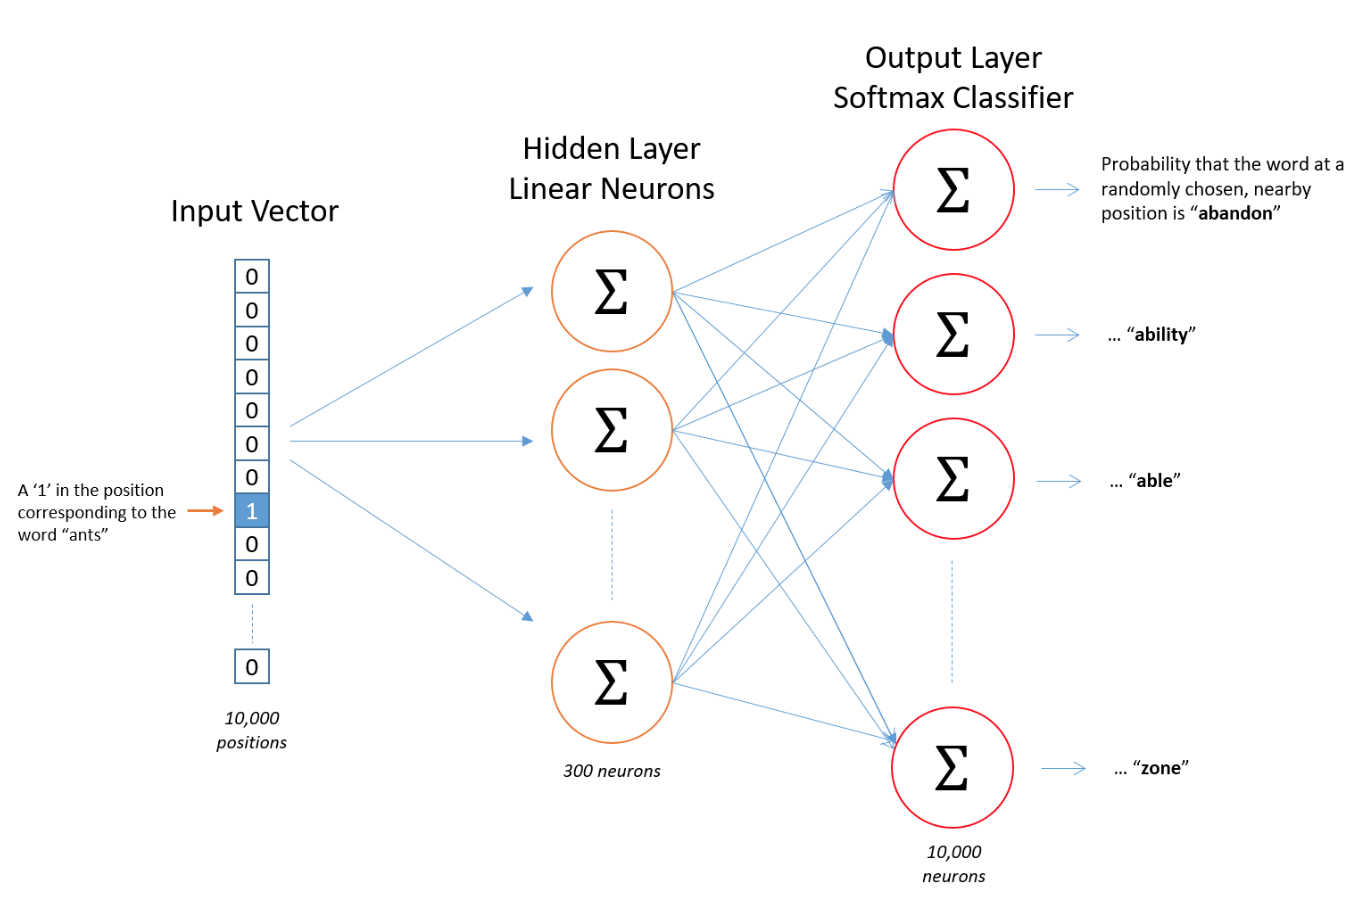
\includegraphics[width=\columnwidth]{images/w2v-structure.png}
	\caption{Structure of Word2vec Network
		}\label{fg:w2v-structure}\cite{w2v-tutorial}
\end{figure}

The input vector is an one-hot vector of length 10000, where only one entry 
is 1 and all others are 0. This vector indicates which input word it represents. 
(Notice there is a one-to-one relationship between the input vector and each 
word in the vocabulary). The hidden layer of size 300, is basically a 
$10000\times 300$ matrix where each role is representing each word in the 
vocabulary in a form of a 300-length real-valued vector. Notice that this 
matrix is what we will save as the ultimate output of our word2vec task, since 
it is the word embeddings for each word. The output of the network is just 
used to tune the numbers in this matrix by comparing with the ground truth. 
(This is why some authors refers this neural network task as a fake task 
\cite{w2v-tutorial}). The output layer which contains the same number of 
neurons as the vocabulary size, is basically a matrix of dimension $300\times 
10000$. By a simple linear algebra calculation we know that taken one input 
vector, the network will output a vector of 10000. After a softmax activation 
function, which normalize these 10000 numbers to a discrete probability 
distribution, we get the probability that each word appear in the context of 
the input word. The loss function could be defined comparing the distance of 
this distribution with the one represented by the ground truth (as provided 
by the training data). 

Training the network involves using techniques such as back propagation to 
minimize the loss function by alternating the weights in the two matrices 
discussed above. 

\subsection{Practical Techniques} 
The word2vec model with a large vocabulary could be very hard to train due 
to the extremely high dimensionality. Mikolov et al discussed several practical 
techniques on top of the basic model above 
\cite{DBLP:journals/corr/MikolovSCCD13}.  There are three innovations in this 
second paper, also discussed by Chris McCormick in his online tutorial 
\cite{w2v-tutorial}, the author will list them below without detailed 
explanation.
\begin{enumerate}
	\item Treating common word pairs or phrases as single “words” in their 
	model.
	\item Subsampling frequent words to decrease the number of training 
	examples.
	\item Modifying the optimization objective with a technique they called 
	“Negative Sampling”, which causes each training sample to update only a 
	small percentage of the model’s weights.
\end{enumerate}

\subsection{Intuition and Implementation}

Using word embeddings such as word2vect representing each word a vector 
provides the syntactic and semantic information about the words which in 
turn can be used for various other tasks. Words which are similar to each 
other are more likely to have similar context therefore the embedding vectors 
are closer in distance. This is the intuition of the model. 

The author did not implement the word2vec model from scratch. Instead, the 
library gensim provides the word2vec model that one could train on his own 
corpus. The word vector for each token can be then provided. The sample 
code is attached here:

 \begin{lstlisting}[language=Python]
import gensim

def train_w2v(sent_list, size=300):
		model = gensim.models.Word2Vec(sent_list, min_count=1,size=size)
		model.delete_temporary_training_data(replace_word_vectors_with_normalized=True)
		return model

def token2vec(token,w2vmodel):
		return w2vmodel.wv[token]
\end{lstlisting}


\section{POS Tagging Using Scikit-learn}
\label{s:pos-sklearn}

This section explains using the library scikit-learn to train a POS tagger with 
hand extracted feature and word embeddings. Different machine learning 
models are applied and the accuracy is around 95\% for hand extracted 
features but relatively low for word embeddings (below 70\%). These could 
be used as a baseline for advanced taggers introduced in Section 
\ref{s:LSTM}. 

\subsection{Data}

The data set I am using for this part is the Treebank tagged sentences 
included in the NLTK (Natural Language Toolkit) package. This is only a small 
fraction (10\%) of the Penn Treebank corpus, which contains 3914 tagged 
sentences and 100676 tagged tokens. For only learning purpose, I did not try 
to purchase the full Penn Treebank. Another option is the Brown corpus, 
which contains 57340 tagged sentences and a vocabulary of 56057. 

Another reason that I am using the Treebank tagged sentences but not the 
Brown corpus for this part is that due to some unknown limitation of 
scikit-learn (and perhaps my machines), training the neural network on 80\% 
of the Treebank data already causes resource issues. Therefore I can only 
reduce the training proportion to 70\%. In Section\ref{s:LSTM}, I used both 
Treebank and Brown because keras running tensorflow backend has no 
problem even handling Brown Corpus. 

\subsection{Method1: hand crafted features}
As a baseline, I tried to extract some very simple features on each token as 
the input for various models. These features include:
\begin{itemize}
	\item the token itself
	\item if the token is the start of the sentence
	\item if the token is the last of the sentence
	\item if the token is capitalized
	\item if the token has only capital letters
	\item if the token has only lower letters
	\item 3 prefix of the word
	\item 3 suffix of the word
	\item the previous word
	\item the next word
	\item if the word has hyphen
	\item if the word is numeric
	\item if the word has a capitalized word inside (not the first letter)
\end{itemize}

I used the machine learning models in scikit-learn to perform the training on 
70\% of the data and test on the rest. The models include decision tree, 
random forest and MLP (feedforward networks) with different number of 
hidden layers and units. After playing around with different parameters, 
based on these hand crafted features, all models could achieve accuracy 
around 94\% to 95\%. 

For MLP in particular, using one hidden layer of 200 neurons achieve 
accuracy of 95.3\%, using two hidden layers (50,50) achieve accuracy of 
95.0\% and using two hidden layers (800,30) achieve 95.2\% accuracy. 
Varying different number of neurons in each layers, alternating activation 
functions, and playing around with other parameters do not seem to improve 
the results. Therefore I believe the limit of using this set of features are 
around 95\% accuracy. 

\subsection{Method2: using word vectors}
In the second method, instead of extracting features, I use the word vectors 
out of the word2vec model (trained on the same corpus) as the features. I 
chose the vector dimension to be 300 (as Google did) and concatenated the 
vector of the chosen word with the previous and next words. This results in 
a feature vector of 900 in length. 

However, using this as the input to the same models yield very poor results. 
For decision tree and random forest, the accuracy is around 40\%. Since the 
word2vec model is calculated from neural networks, I tried to test many 
different structures of feedforward networks, the results of accuracy are 
summarized in the Table \ref{t:results-nn1}, Table \ref{t:results-nn2} and 
Table \ref{t:results-nn3}.
\begin{table}[!ht]
	\centering
	\caption{Accuracy for Feedforward Network Using Word 
	Vectors I}\label{t:results-nn1}
	\begin{tabular}{llll}
		\hline \hline 
		Model Number & Number of Hidden layers & Size of Hidden Layers 
		&Accuracy\\
		\hline
		1 & 1 & (100) &   53.85\%   \\
		2 & 1 & (200) &   55.25\%   \\
		3 & 1 & (500) &   56.27\%   \\
		4 & 1 & (1000) &   58.90\%   \\
		5 & 1 & (1500) &   59.47\%   \\
		6 & 1 & (2000) &   60.24\%   \\
		7 & 1 & (2500) &   58.26\%   \\
		8 & 1 & (3000) &   55.77\%   \\
		9 & 1 & (3500) &   56.34\%   \\
		10 & 1 & (4000) &   57.46\%   \\
		11 & 1 & (4500) &   56.83\%   \\
		12 & 1 & (5000) &   57.50\%   \\
		13 & 1 & (5500) &   58.54\%   \\
		\hline \hline 
	\end{tabular}
\end{table}

Table \ref{t:results-nn1} shows the results by using only 1 hidden layer. By 
increasing the number of neurons in that layer, the accuracy increases at 
first. After 2000 neurons, increasing the size of the layer does not increase 
accuracy any more. In all the accuracy is around or below 60\%.

\begin{table}[!ht]
	\centering
	\caption{Accuracy for Feedforward Network Using Word 
		Vectors II}\label{t:results-nn2}
	\begin{tabular}{llll}
		\hline \hline 
		Model Number & Number of Hidden layers & Size of Hidden Layers 
		&Accuracy\\
		\hline
		1 & 2 & (3000, 100) &   58.78\%   \\
		2 & 2 & (3000, 200) &   59.67\%   \\
		3 & 2 & (3000, 500) &   63.61\%   \\
		4 & 2 & (3000, 1000) &   64.72\%   \\
		5 & 2 & (3000, 1500) &   61.60\%   \\
		6 & 2 & (3000, 2000) &   62.38\%   \\
		7 & 2 & (3000, 2500) &   65.28\%   \\
		8 & 2 & (3000, 3000) &   68.72\%   \\
		9 & 2 & (3000, 3500) &   65.40\%   \\
		10 & 2 & (3000, 4000) &   60.81\%   \\
		11 & 2 & (3000, 4500) &   59.43\%   \\
		12 & 2 & (4000, 3000) &   59.70\%   \\
		13 & 2 & (4000, 4000) &   61.86\%   \\
		14 & 2 & (4000, 5000) &   65.29\%   \\
		15 & 2 & (5000, 3000) &   64.63\%   \\
		16 & 2 & (5000, 4000) &   62.99\%   \\
		17 & 2 & (5000, 5000) &   66.13\%   \\
		\hline \hline 
	\end{tabular}
\end{table}

Table \ref{t:results-nn2} shows accuracy of models with 2 hidden layers. The 
results are generally better than the ones with only one hidden layer. 
However there is no obvious patterns about how different number of 
neurons could affect the accuracy. The highest so far is to use two layers 
each having 3000 neurons. 

\begin{table}[!ht]
	\centering
	\caption{Accuracy for Feedforward Network Using Word 
		Vectors III}\label{t:results-nn3}
	\begin{tabular}{llll}
		\hline \hline 
		Model Number & Number of Hidden layers & Size of Hidden Layers 
		&Accuracy\\
		\hline
		1 & 3 & (3000, 3000, 3000) &   63.68\%   \\
		2 & 3 & (3000, 3000, 4000) &   54.90\%   \\
		3 & 3 & (3000, 3000, 5000)&   69.44\%   \\
		4 & 4 & (3000, 3000, 3000, 3000) &   51.80\%   \\
		5 & 4 & (3000, 3000, 3000, 4000) &   57.62\%   \\
		\hline \hline 
	\end{tabular}
\end{table}

Table \ref{t:results-nn3} shows accuracy of models with 3 or more hidden 
layers. The results are not better than the ones with two hidden layer. 

\begin{remark}
	The results of these model are in general performing much worse 
	compared to the baseline with hand crafted features. The reason is 
	probably that the word vector of three words may not be able to provide 
	enough information for part of speech. Although the hand crafted 
	features did not include more words in the sequence (also the previous 
	and the next), they have more other features such as prefix, suffix, and  
	word-shape. These features may not be well-represented by the word 
	vectors. Another possibility is that feedforward network is not well applied 
	to this type of inputs. In Section \ref{s:LSTM}, we can show that using 
	RNN could achieve a much better result. 
\end{remark}

\begin{remark}
	The accuracy results in the previous three tables are only from one run of 
	the corresponding model. More iterations or techniques like 
	cross-validation are not used because the training process is very 
	time-consuming. On average, each model takes more than 3 hours to 
	train. I suppose the inefficiency is due to the implementation of 
	scikit-learn, which is a machine learning library but not one specialized for 
	deep learning. In fact, when using keras (with a scikit-learn wrapper), the 
	same model runs within 30 minutes. 
\end{remark}

\begin{remark}
	Another limitation of scikit-learn is that when handling more than 75000 
	training tokens, python will show errors with memory limitation. However, 
	same model using keras (with a scikit-learn wrapper) can be executed 
	without problems.
\end{remark}


\section[POS Using BLSTM-RNN in Keras]{POS Tagging Using Bidirectional 
Long Short-Term Memory Recurrent Neural Network }
\label{s:LSTM}
This section shows the steps and results for using a type of recurrent neural 
network: Long Short-Term Memory to tag part of speech. The library used 
for implementation is keras, which is ``a high-level neural networks API, 
written in Python and capable of running on top of TensorFlow, CNTK, or 
Theano. It was developed with a focus on enabling fast experimentation. 
Being able to go from idea to result with the least possible delay is key to 
doing good research'' \cite{keras-doc}.

\subsection{Previous Models Revisit Using Keras}
All the models in Section \ref{s:pos-sklearn} can be implemented in keras 
using a tensorflow backend. There are two ways for the implementation. The 
first is to use a wrapper for scikit-learn so that most of the code in previous 
scikit-learn implementation could be directly applied. The other is to rewrite 
code in keras, which allows more flexibility and options regarding deep neural 
networks. Both methods are tested (which gave similar results) and codes 
are included in the attached github repository. 

Further, when use keras, the more efficient backend allow us to train the 
model on much larger training sets, therefore, the analysis is also applied to 
Brown Corpus. The model performance (using same hand crafted features) 
are displayed in Figure \ref{f:mphc}. Note that I am using a two layer MLP 
with number of hidden units 400 and 300 respectively, details of which is 
shown in Figure \ref{f:mhc}
\begin{figure}[!ht]
	\centering
	\begin{subfigure}[b]{0.5\textwidth}
		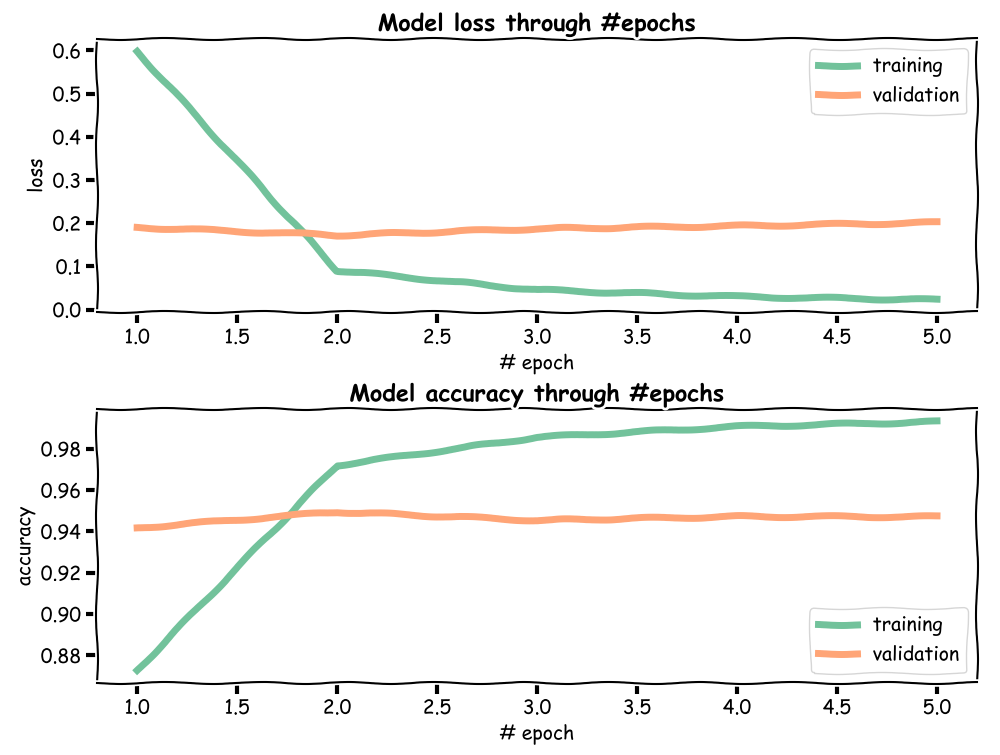
\includegraphics[height=1.9in]{images/model-performance-tree.png}
		\caption{Treebank corpus}
	\end{subfigure}%
	\begin{subfigure}[b]{0.5\textwidth}
		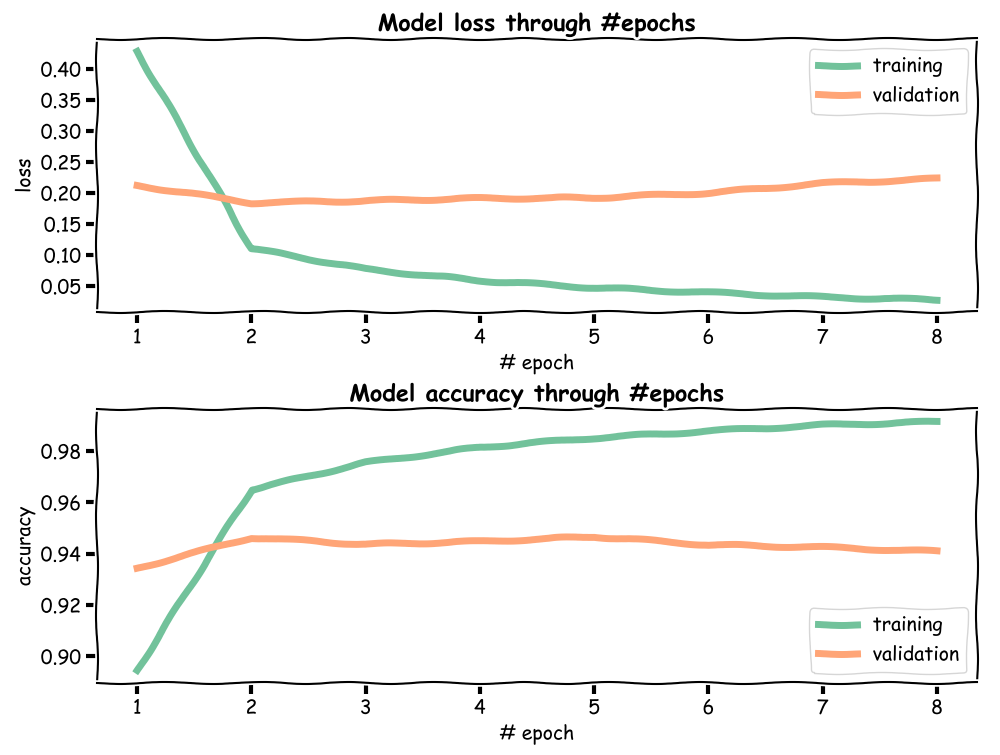
\includegraphics[height=1.9in]{images/model-performance-brown.png}
		\caption{Brown corpus}
	\end{subfigure}
	\caption{Model Performance with Hand Crafted Features and FeedForward 
	NN}\label{f:mphc}
\end{figure}

\begin{figure}[!ht]
	\centering
	\begin{subfigure}[b]{\textwidth}
		\centering
		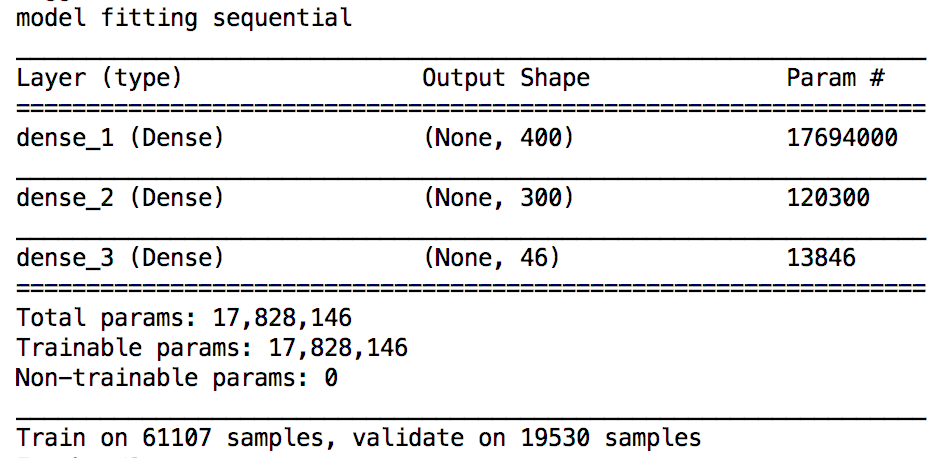
\includegraphics[height=1.5in]{images/model-tree.png}
		\caption{Treebank corpus}
	\end{subfigure}%
   \\
	\begin{subfigure}[b]{\textwidth}
			\centering
		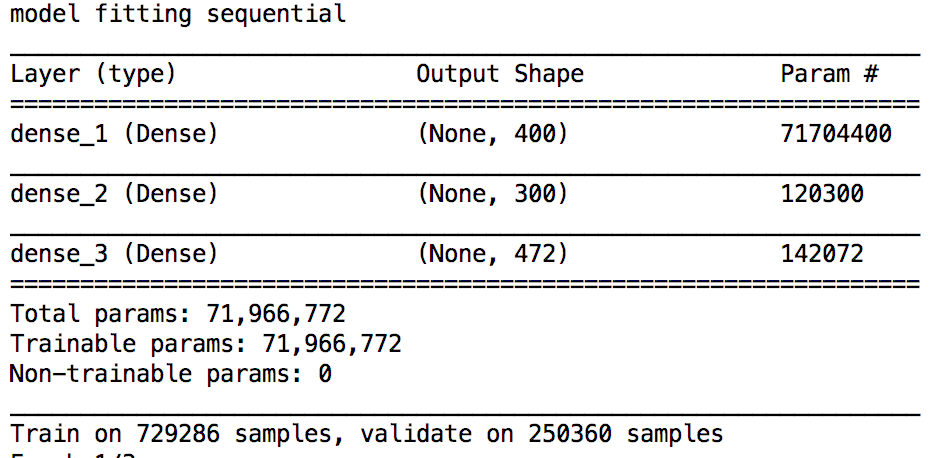
\includegraphics[height=1.5in]{images/model-brown.png}
		\caption{Brown corpus}
	\end{subfigure}
	\caption{Model Used with Hand Crafted Features and FeedForward 
		NN}\label{f:mhc}
\end{figure}

For both corpus, the model performances are very similar. First, the 
accuracy on validation sets is above 94\%. Second, after two epochs, the 
model seems to start overfitting. The final accuracy on test sets (stopped 
after 3 epochs) are 95.17\% and 95.68\%. 

Similar, using the word2vec embeding and feedfarward networks in keras 
yield similar results as before, no more than 70\%. The details are omitted 
here since the performance is not good. 

\subsection{Bidirectional Long Short-Term Memory Recurrent Neural 
Network}
``In theory, RNNs are absolutely capable of handling  long-term 
dependencies. Sadly, in practice, RNNs don’t seem to be able to learn them'' 
\cite{olah-blog-lstm}. Therefore, some researchers have suggested using a 
special gated recurrent neural network to handle POS tagging 
\cite{Wang2015PartofSpeechTW}. In this subsection, the author summarized 
some of the main features of LSTM RNN, inspired by Christopher Olah 
\cite{olah-blog-lstm}. The comparison can be illustrated by Figure 
\ref{f:lstmrnn}.

\begin{figure}[!ht]
	\centering
	\begin{subfigure}[b]{\textwidth}
		\centering
		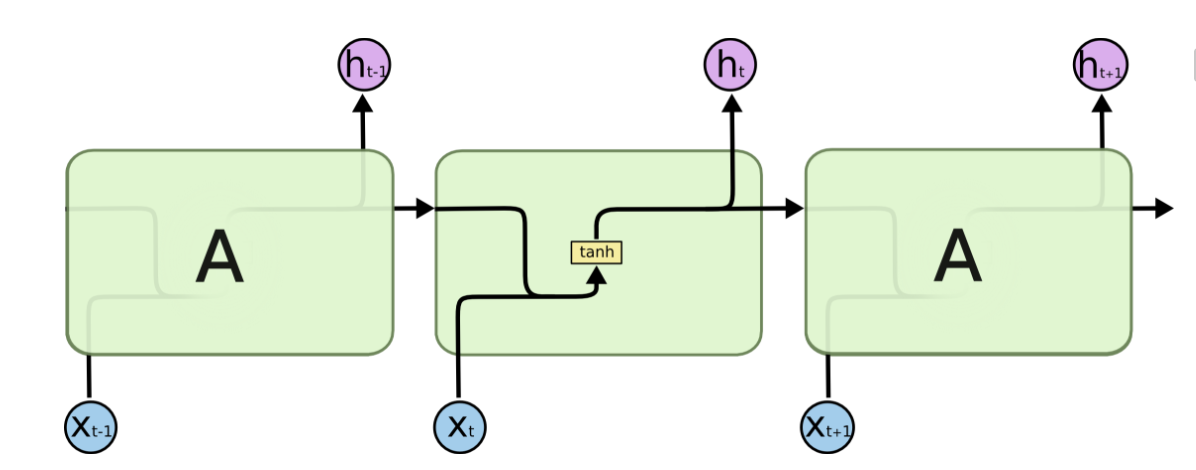
\includegraphics[height=1.9in]{images/standardRNN.png}
		\caption{Standard RNN contains a single layer}
	\end{subfigure}%
	\\
	\begin{subfigure}[b]{\textwidth}
		\centering
		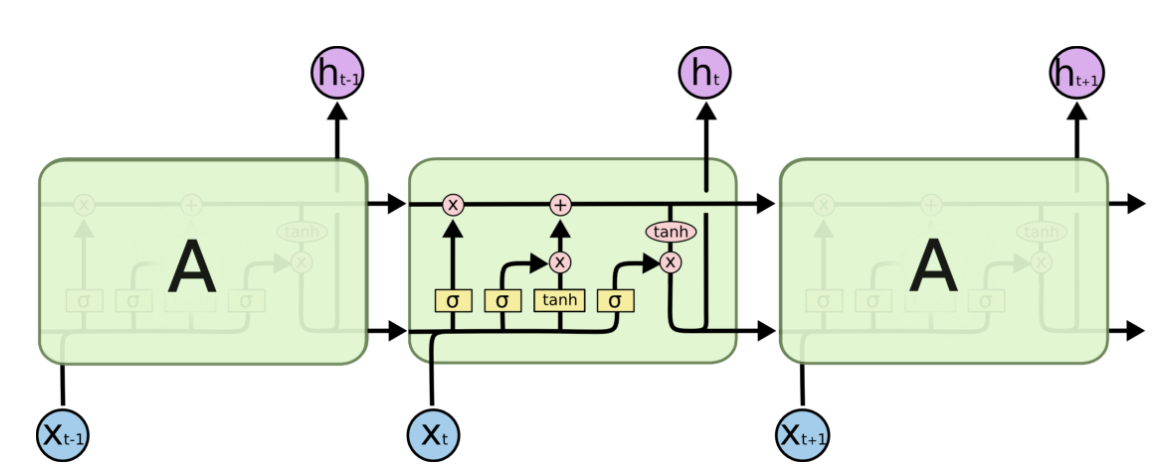
\includegraphics[height=1.9in]{images/lstmRNN.png}
		\caption{LSTM contains four interacting layers}
	\end{subfigure}
	\caption{The repeating module in RNN}\label{f:lstmrnn}\cite{olah-blog-lstm}
\end{figure}

In standard RNNs, the repeating module will have a very simple structure, 
such as a single tanh layer, or relu layer etc. However, in LSTM, the repeating 
module consists of several gates that controls the probability of information 
flow thus deciding to keep or abandon long/short memories. The details of 
the structure within the repeating units is as in Figure \ref{f:lstmgates} where 
the 3 equations on the right-hand side correspond to forget gate, input gate, 
and output gate respectively.  
\begin{figure}[!ht]
	\centering
	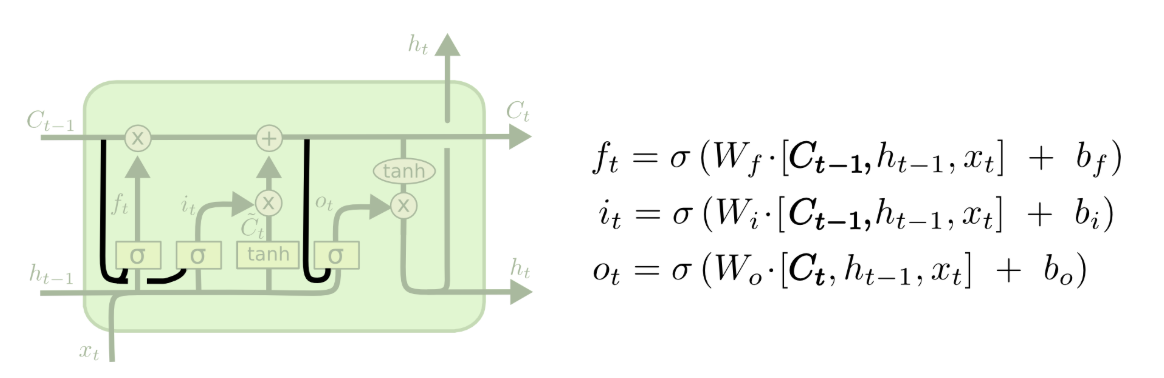
\includegraphics[width=\columnwidth]{images/LSTMgates.png}
	\caption{LSTM Repeating Module Gates in 
	Details}\label{f:lstmgates}\cite{olah-blog-lstm}
\end{figure}

\begin{itemize}
	\item Forget gate: $f_t=\sigma(W_f\dot [C_{t-1},h_{t-1},x_t]+b_f)$, where 
	the weights ($W_f$) are applied to previous hidden state ($C_{t-1}$), 
	previous output $h_{t-1}$, and the current input ($x_t$), plus a bias term 
	($b_f$). After a sigmoid activation function ($\sigma$), $f_t$ is 
	transformed to a number between 0 and 1, representing the fraction of 
	previous memory to keep. 
	\item Input gate: $i_t=\sigma(W_i\dot [C_{t-1},h_{t-1},x_t]+b_i)$, where a 
	new sets of weights and bias are applied to the same features as before, 
	out put a fraction of current input to be taken into consideration.
	\item Output gate: $o_t=\sigma(W_o\dot [C_{t},h_{t-1},x_t]+b_o)$, where 
	another new sets of weights and bias are applied to the same features as 
	before (except using current cell state $C_t$), output a fraction of current 
	output to be emit. 
\end{itemize}

 By using the three gates above, we can update the old cell state $C_{t-1}$ to 
 current cell state $C_t$ by the following two steps. The step one is 
 calculating the input (before input gate):
 \[
 \tilde{C_t}=\tanh (W_C\dot [h_{t-1},x_t]+b_C)
 \]
 Then current cell state is updated according to input gate and forget gate:
 \[
 C_t=f_t\,C_{t-1}+i_t\,\tilde{C_t}
 \]
The output of the current cell is then:
\[
h_t=o_t\, \tanh(C_t)
\]

Another illustration from Goodfellow's book is in Figure 
\ref{f:lstmgatesgood}, ``where an input feature is computed with a regular 
artificial neuron unit. Its value can be accumulated into the state if the 
sigmoidal input gate allows it. The state unit has a linear self-loop whose 
weight is controlled by the forget gate. The output of the cell can be shut off 
by the output gate. All the gating units have a sigmoid nonlinearity, while the 
input unit can have any squashing nonlinearity. The state unit can also be 
used as an extra input to the gating units. The black square indicates a delay 
of a single time step'' \cite{Goodfellow-et-al-2016}.

\begin{figure}[!ht]
	\centering
	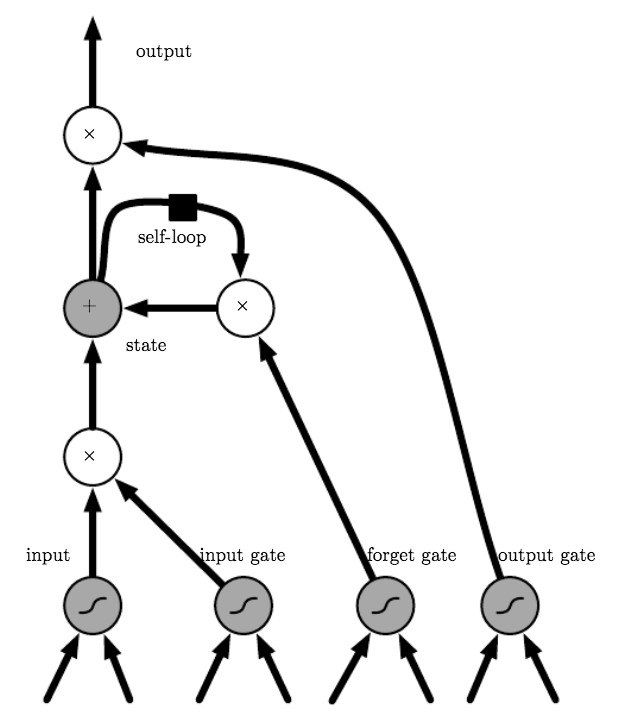
\includegraphics[height=3in]{images/lstm-goodfellow.png}
	\caption{LSTM Repeating Module Gates in 
		Deep Learning Text 
		Book}\label{f:lstmgatesgood}\cite{Goodfellow-et-al-2016}
\end{figure}

Furthermore, we use bidirectional LSTM RNN instead of unidirectional as 
suggested by Wang and his co-authors \cite{Wang2015PartofSpeechTW}. 
They also mentioned that: as a neural network model, it is awkward
for BLSTM RNN to make use of conventional NLP features, such as 
morphological features. Word embeddings seem to be a better choice. 
Therefore, I used word2vec model as discussed in Section \ref{s:w2v} as the 
input. 

\subsection{Network Structure and Implementation}
The implementation includes adding three layers in keras model building to 
construct the network: 
\begin{enumerate}
	\item Embedding Layer: applying word2vec and transform the tokens into 
	a real valued vector with a fixed length. 
	\item Bidirectional​ ​LSTM​ ​layer
	\item Fully Connected Layer: a simple output layer using softmax to 
	convert the vector to probability values for each tagging (similar as the 
	output layer of word2vec network).
\end{enumerate}
The structure is illustrated in Figure \ref{f:fullstructure}, in Aneesh's Github 
repository documentation \cite{aneesh-joshi-LSTM-POS-Tagger}.
\begin{figure}[!ht]
	\centering
	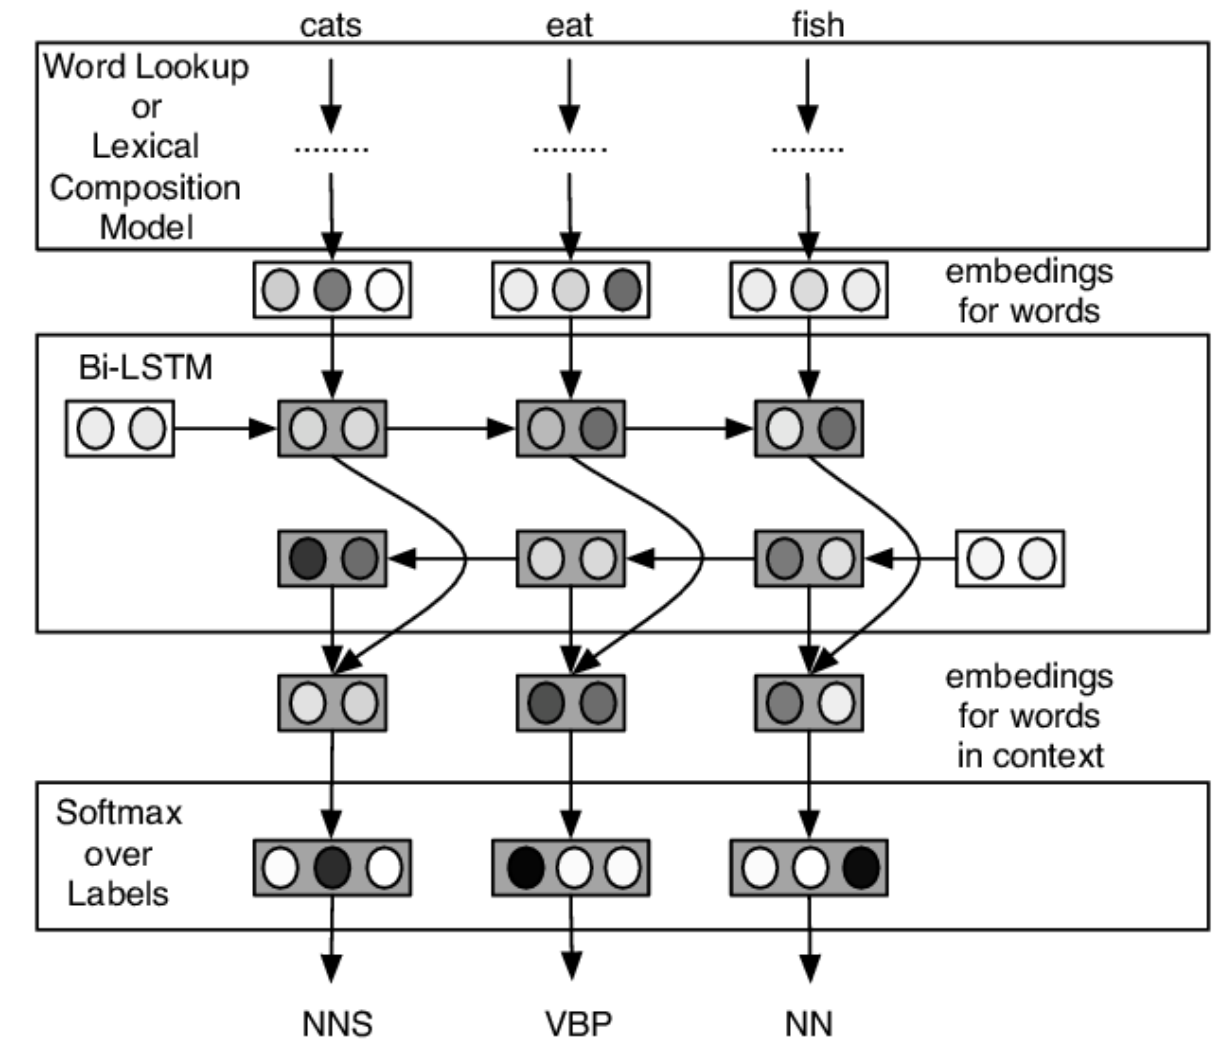
\includegraphics[height=5in]{images/POS-structure.png}
	\caption{Structure of the 
	Network}\label{f:fullstructure}\cite{aneesh-joshi-LSTM-POS-Tagger}
\end{figure}

Note that since all the sentences are not of the same length, it creates a lot 
of variability and creates a staggered matrix/tensor which isn’t good for fast 
training in the TensorFlow paradigm. Therefore, Aneesh padded all the words 
with zeros in the beginning to make all the sentences have the same 
dimension and for sentences of length longer than 100, we just simply 
truncated the sentence and discard the tokens after 100. 

The code for implementing the structure depicted in Figure 
\ref{f:fullstructure} is extremely simple in keras. The sample code is attached 
as follows:

 \begin{lstlisting}[language=Python]
embedding_layer = Embedding(len(word2int) + 1,
												EMBEDDING_DIM,
												weights=[embedding_matrix],
												input_length=MAX_SEQUENCE_LENGTH,
												trainable=True)
												
sequence_input = Input(shape=(MAX_SEQUENCE_LENGTH,), dtype='int32')

embedded_sequences = embedding_layer(sequence_input)

l_lstm = Bidirectional(LSTM(64, 	
								  return_sequences=True))(embedded_sequences)
								  
preds = TimeDistributed(Dense(len(tag2int) + 1, activation='softmax'))(l_lstm)

model = Model(sequence_input, preds)
model.compile(loss='categorical_crossentropy',
						optimizer='rmsprop',
						metrics=['acc'])
\end{lstlisting}


\subsection{Results}

The discussed BILSTM RNN structure is implemented in keras with 
TensorFlow backend. Again, the model is applied to the smaller Treebank 
corpus and the larger Brown corpus. Across the task, 60\% of the data is 
used as training, with 20\% validation and 20\% testing. The model 
performance are displayed in Figure \ref{f:mpw2v} with the detailed network 
model summarized in Figure \ref{f:mw2v}
\begin{figure}[!ht]
	\centering
	\begin{subfigure}[b]{0.5\textwidth}
		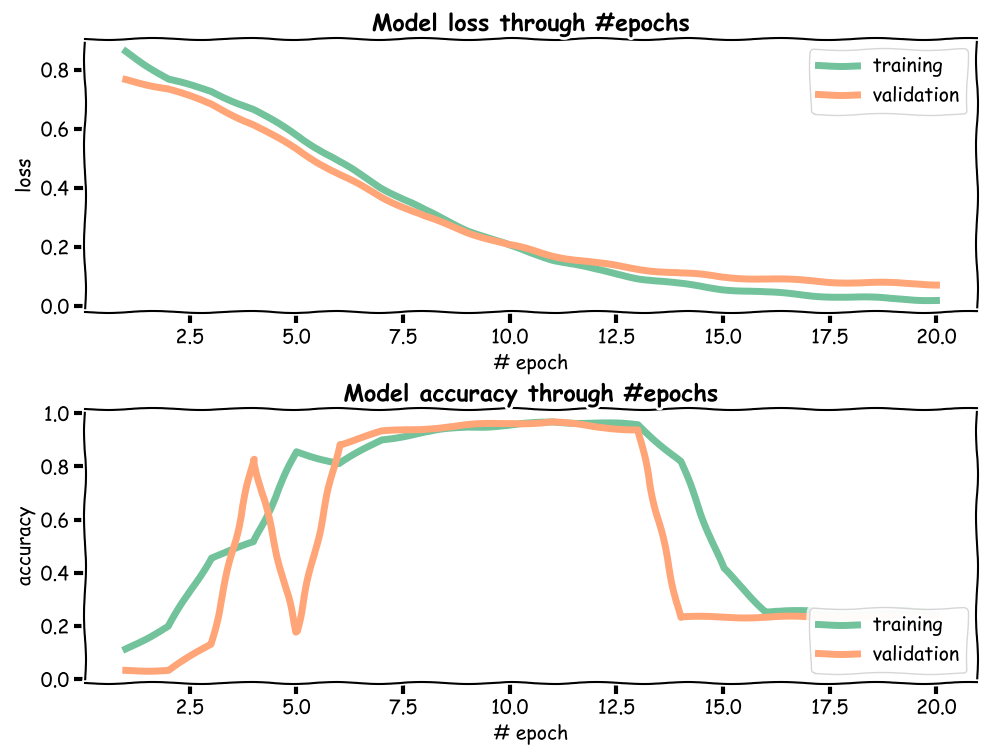
\includegraphics[height=1.9in]{images/model-performance-lstm-tree.png}
		\caption{Treebank corpus}
	\end{subfigure}%
	\begin{subfigure}[b]{0.5\textwidth}
		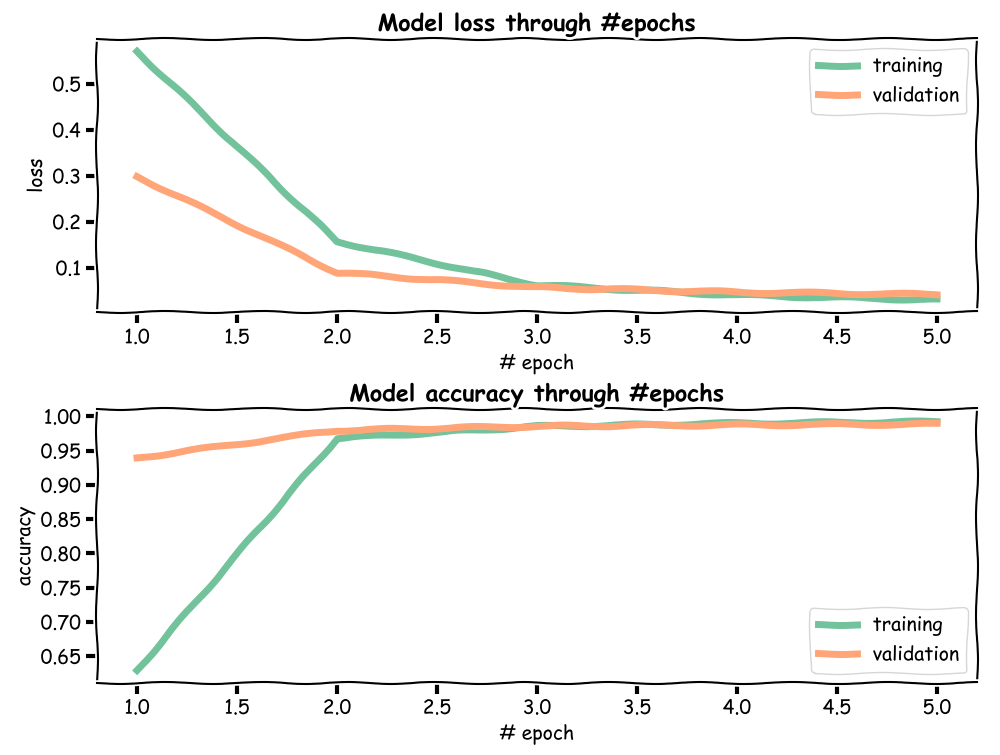
\includegraphics[height=1.9in]{images/model-performance-lstm-brown.png}
		\caption{Brown corpus}
	\end{subfigure}
	\caption{Model Performance with Word2vec Embeddings and BI-LSTM 
	RNN}\label{f:mpw2v}
\end{figure}

\begin{figure}[!ht]
	\centering
	\begin{subfigure}[b]{\textwidth}
		\centering
		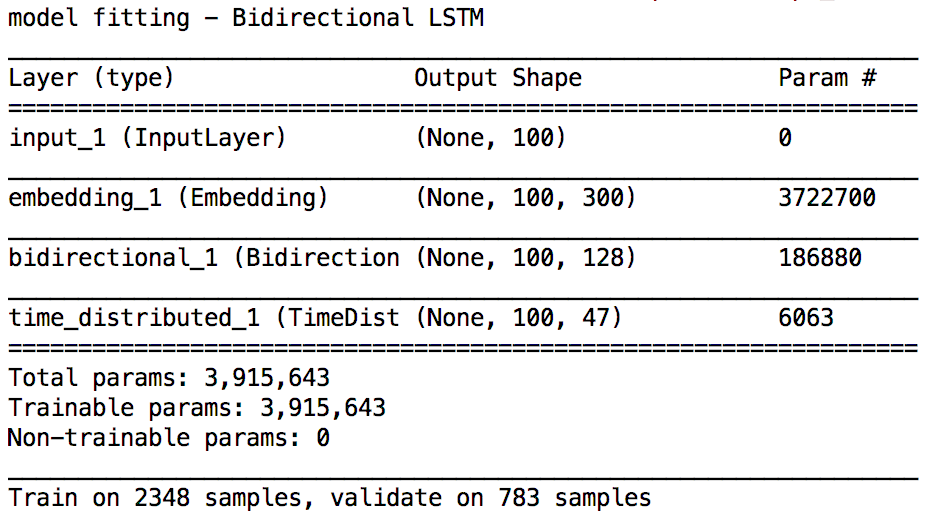
\includegraphics[height=1.5in]{images/model-lstm-tree.png}
		\caption{Treebank corpus}
	\end{subfigure}%
	\\
	\begin{subfigure}[b]{\textwidth}
		\centering
		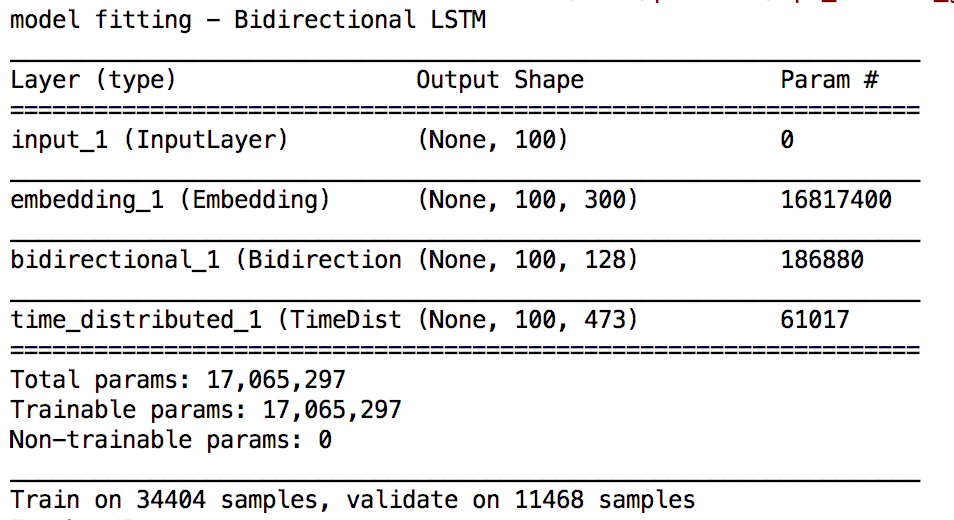
\includegraphics[height=1.5in]{images/model-lstm-brown.png}
		\caption{Brown corpus}
	\end{subfigure}
	\caption{Model Used  with Word2vec Embeddings and BI-LSTM 
	RNN}\label{f:mw2v}
\end{figure}

For the Treebank corpus, the model performance shows that the model is 
underfitting before epoch 7 and overfitting after epoch 13. The accuracy 
on final test set, after stopping at the 13th epoch, is 97.31\%. 

For Brown corpus, the model performance looks more stable in terms of 
training and validation accuracy over epochs. The 
accuracy on validation sets is above 98\% and after two epochs, the 
model seems to start overfitting. The final accuracy on test sets (stopped 
after 3 epochs) is 98.57\%, which is consistent with the references: 98.79\% 
from Aneesh \cite{aneesh-joshi-LSTM-POS-Tagger}. Wang et al 
\cite{Wang2015PartofSpeechTW} showed a lower accuracy of 97.4\% 
because they are training one one corpus and testing on another one, which 
requires higher generalization of the trained tagger. However, in my case, the 
Treebank corpus (46 different tags) and the Brown corpus (472 different 
tags) have different tagging convention, therefore I keep the training and 
testing within one corpus thus having a higher accuracy. Accuracy over 98\% 
on a blind test set is very impressive and demonstrates the power of deep 
learning techniques used including word2vec, and BI-LSTM RNN. 


\section{Conclusion}
\label{s:conclusion}

In this independent study, the author followed the guidance of Prof. Damir 
Cavar and focused on basic knowledge of deep learning and possible 
application to natural language processing. A good fraction of study time is 
distributed to read the Goodfellow's deep learning text book and try to 
understand different deep neural network architecture and techniques. In 
application, the author chose part-of-speech tagging, the very basic 
component in NLP and experiment using different Python libraries 
(Scikit-learn, TensorFlow, Keras) with both hand crafted features and 
self-trained word embeddings using word2vec models. 

It appears that the deep learning library Keras is more efficient and flexible 
for designing and training complicated neural network models with large data 
sets. For POS tagging, hand crafted features with various machine learning 
algorithms could achieve accuracy around 95\%. Using word embeddings 
from word2vec as features tend to result in low accuracy (below 70\%) when 
trained with feedforward networks. However, using a special kind of 
recurrent neural network: bidirectional long-short term memory recurrent 
neural network, the accuracy is very high, over 97\% for part of the Treebank 
Corpora and over 98\% for the Brown Corpus. 

\paragraph{Future research areas} Due to time constraint, the author did 
not have enough time to experiment through many options provided by the 
Keras library to improve or compare different architecture. Further, other 
than POS tagging, deep learning techniques have been applied to many other 
NLP tasks. The author would like to try different deep network structures to 
improve accuracy in areas such as parsing, co-reference resolution, 
sentiment analysis and applications with knowledge graph. 

\paragraph{Acknowledgement }The author would like to thank Prof. Damir 
Cavar for his support and suggestions throughout the independent study 
and illustrations and materials regarding deep learning. 

\pagebreak

\appendix
\section{Code Files Index}
The code for this project is included in the Github repository: 
\url{https://github.com/minchen57/deeplearningNLP}
There are several Python source code in this folder and they correspond to 
the following tasks mentioned in this report:

\begin{table}[!ht]
	\centering
	\caption{Source Code Files}\label{t:code}
	\begin{tabular}{llll}
		\hline \hline 
		File Name & Libraries & Features & Model \\
		\hline
		\verb|POS_scikitlearn.py| & Scikit-learn & hand crafted & DT, RF, NN \\
		\verb|POS_w2v_scikitlearn.py|& Scikit-learn & word2vec & DT, RF,NN\\
		\verb|POS_keras_scikitlearnwrapper.py|& Keras, Scikit-learn& 
		hand crafted & DT, RF, NN) \\
		\verb|POS_keras.py||& Keras& hand crafted & NN  \\
		\verb|POS_w2v_keras.py|& Keras& word2vec & NN\\
		\verb|POS_LSTM_keras_w2v.py|& Keras& word2vec & BI-LSTM RNN\\
		\hline \hline 
	\end{tabular}
\end{table}

\pagebreak

\bibliographystyle{abbrv}
\bibliography{report} 

\end{document}
